\documentclass[12pt]{article}
\usepackage{amsmath}
\usepackage[lmargin = 1in, rmargin = 1in, tmargin = 1in, bmargin = 1in]{geometry}
\usepackage[none]{hyphenat}
\usepackage{graphicx}
\usepackage{subcaption}
\usepackage{float}

\title{\textbf{ME598/494 Homework 5}}
\author{Aditya Vipradas\\ASU ID: 1209435588}
\begin{document}
\maketitle
SQP algorithm is implemented to solve the given optimization problem with two inequality constraints. The starting point is considered to be (1, 1). This algorithm is accompanied with the BFGS method to approximate the Hessian of the Lagrangian and the Armijo line search with the corresponding merit function. The active-set strategy is incorporated to solve the QP subproblem in each iteration. As observed from the output, the problem is solved in 4 iterations. Only the first inequality constraint is found to be active and the minimum is obtained at (1.0604, 1.4563). The SQP path and convergence plots are shown below followed by the MATLAB codes.
\begin{figure}[H]
\begin{center}
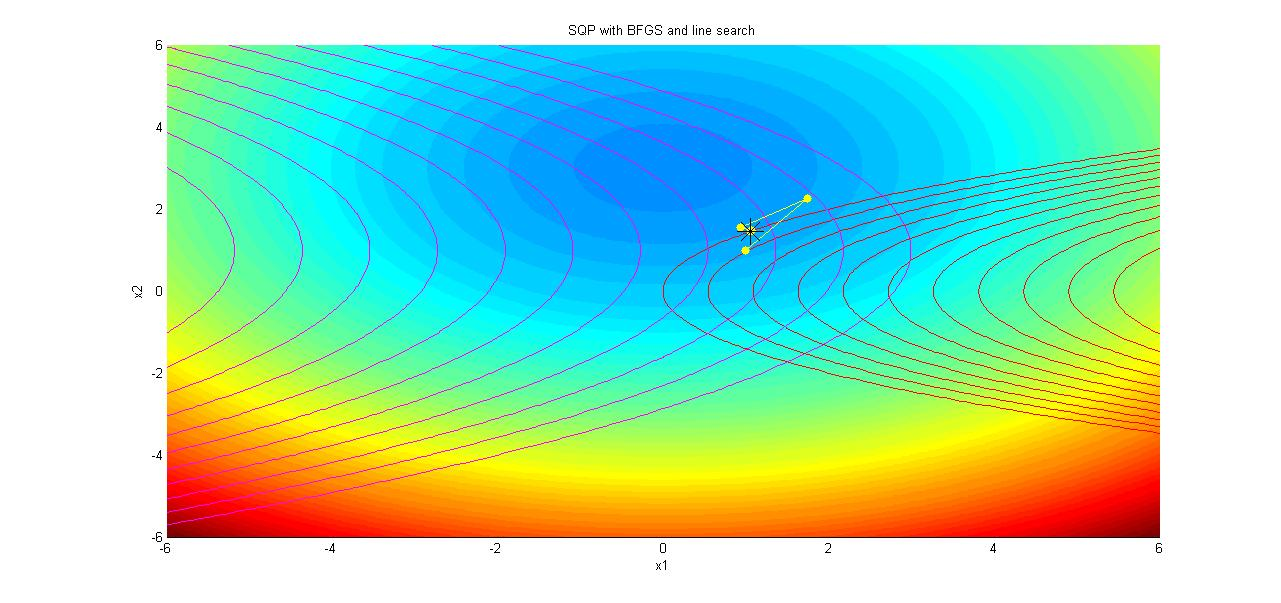
\includegraphics[scale=0.35]{1.jpg}
\caption{SQP (with BFGS and line search) path}  
\end{center}
\end{figure}
\begin{figure}[H]
\begin{center}
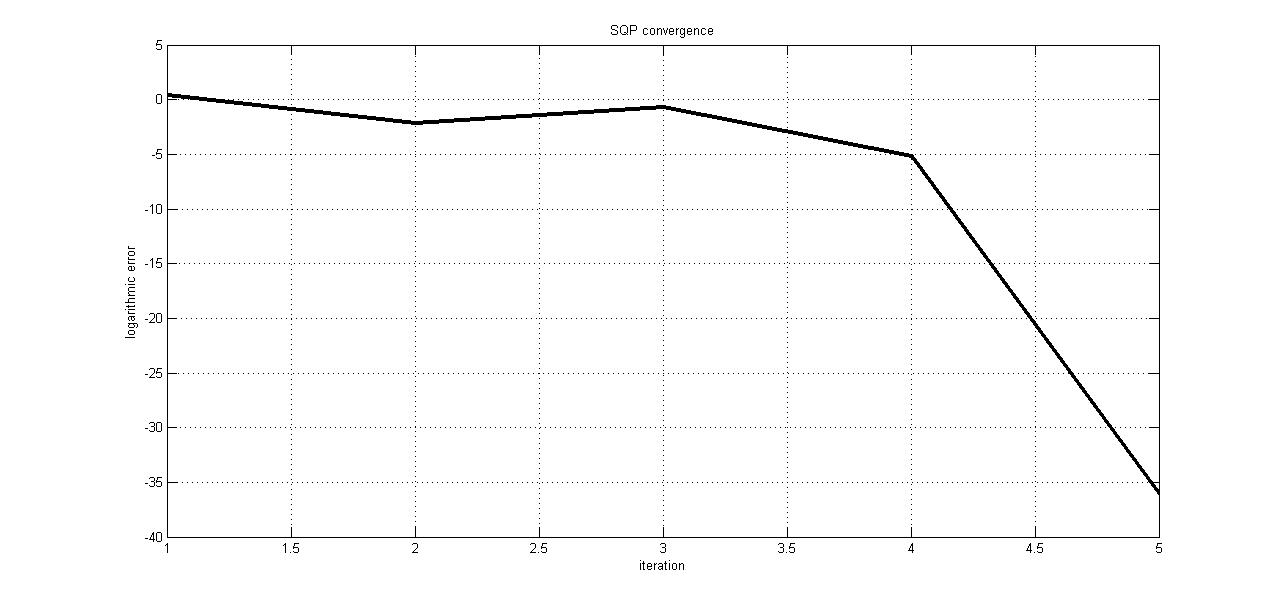
\includegraphics[scale=0.35]{2.jpg}
\caption{Function error plot}  
\end{center}
\end{figure}
\end{document}
